\chapter{Decay Tree Fit}
\label{chap:apdx_dtf}
In complex decay chains, such as \decay{\Lb}{(\decay{\Dz}{\Km\pip})(\decay{\Lz}{\proton\pim})}, typically only the very first particle in the decay chain (\Lb) and the final state particles (\Km, \pip, \proton and \pim) produce signatures in the detector.
In general, the initial particle is produced during the high energetic \proton\proton-scattering which causes a plethora of detector signatures.
Its position is therefore directly reconstructible and referred to as the primary vertex (\gls{pv}), whereas the latter are reconstructed as (charged) tracks from multiple vertices, measured by various detector modules.
The matching of both is ambiguous in general and is additionally impeded by measurement inaccuracies.
A decay tree fit (\gls{dtf}) refines those measurements in one global fit w.r.t.\ a set of constraints and allows an ordering of the different track and \gls{pv} combinations by their respective $\chi^2$ value.
A \gls{dtf} is a fit of constraints\footnote{Technically, at \lhcb the \gls{dtf} is implemented as a Kalman filter, \cf{}~Ref.~\cite{kalmandtf} for more details.} and therefore a correction of the measured track parameters w.r.t.\ given hypotheses.
The measurements are assumed as external constraints with uncertainties, whereas the assumed hypotheses are encoded as strict internal constraints.
A \gls{dtf} without any constraints is pointless and has zero \gls{dof}.
For $n$ measured points and $0<k<n$ constraints the number of parameters is $n-k$ since each constraint can be used to eliminate one measured point by giving it in terms of the remaining measurements.
Hence the \gls{dof} of the $\chi^2$ of the \gls{dtf} is $n-(n-k)=k$.

A \gls{dtf} is used to fit an entire decay chain which can include intermediate states.
Each intermediate state can either be a short-living resonance or an intermediate state with a finite decay length.
Whether or not an intermediate state is considered short- or long-living depends on the detector resolution.
For the \lhcb detector, \jpsi mesons are considered to be short-living, whereas \Dz mesons or \Lz baryons are categorized as long-living intermediate states.
Each intermediate state contributes to the set of constraints by forcing origin- and decay-vertex to be fixed points.
For \decay{\Lb}{(\decay{\Dz}{\Km\pip})(\decay{\Lz}{\proton\pim})} this leads to a set of three constraints, \ie{}, three \gls{dof} in total (\cf{}~Fig.~\ref{fig:detector_decaytops}):
\begin{itemize}
    \item The \proton and \pim tracks should not be skewed. Their common intersection is the decay vertex of the \Lz baryon.
    \item Similarly, both, \Km and \pip, should intersect at the decay vertex of the \Dz meson.
    \item The tracks of the intermediate states \Lz and \Dz that are inferred by four-momentum conservation of the final state particles, should not be skewed lines either, but form the decay vertex of the \Lb baryon. Consequently, this vertex is also the origin vertex of the intermediate states and can be used to determine the lifetime of the respective states.
\end{itemize}
 
For long-living intermediate states that decay via a two-body channel, each vertex constraint contributes one additional \gls{dof} to the $\chi^2$ of the respective \gls{dtf}.
For short-living intermediate states or decay channels with more than two final states the contribution is larger.
For example, the total \gls{dof} of the vertex constraints of a \gls{dtf} of a \decay{\Lb}{(\decay{\jpsi}{\ell^+ \ell^-})(\decay{\Lz}{\proton\pim})} decay sums up to four, since the \jpsi meson is a resonance and thus effectively makes the decay vertex of the \Lb a three point vertex \decay{\Lb}{\ell^+ \ell^- \Lambda} that comes with three \gls{dof}.

Additional constraints can be applied, \eg{}, in most cases it makes sense to constrain the origin vertex of the very first particle of a given decay chain to the \gls{pv} and since this is a fixed point this constraint adds two \gls{dof} to the fit.
Another useful constraint is a mass constraint which forces the invariant mass, given by four-momentum addition of an intermediate state, to match a given particle hypothesis.
Each mass constraint adds one additional \gls{dof} to the fit.
\begin{figure}[htbp]
    \centering
    \begin{subfigure}{.49\textwidth}
        \centering
        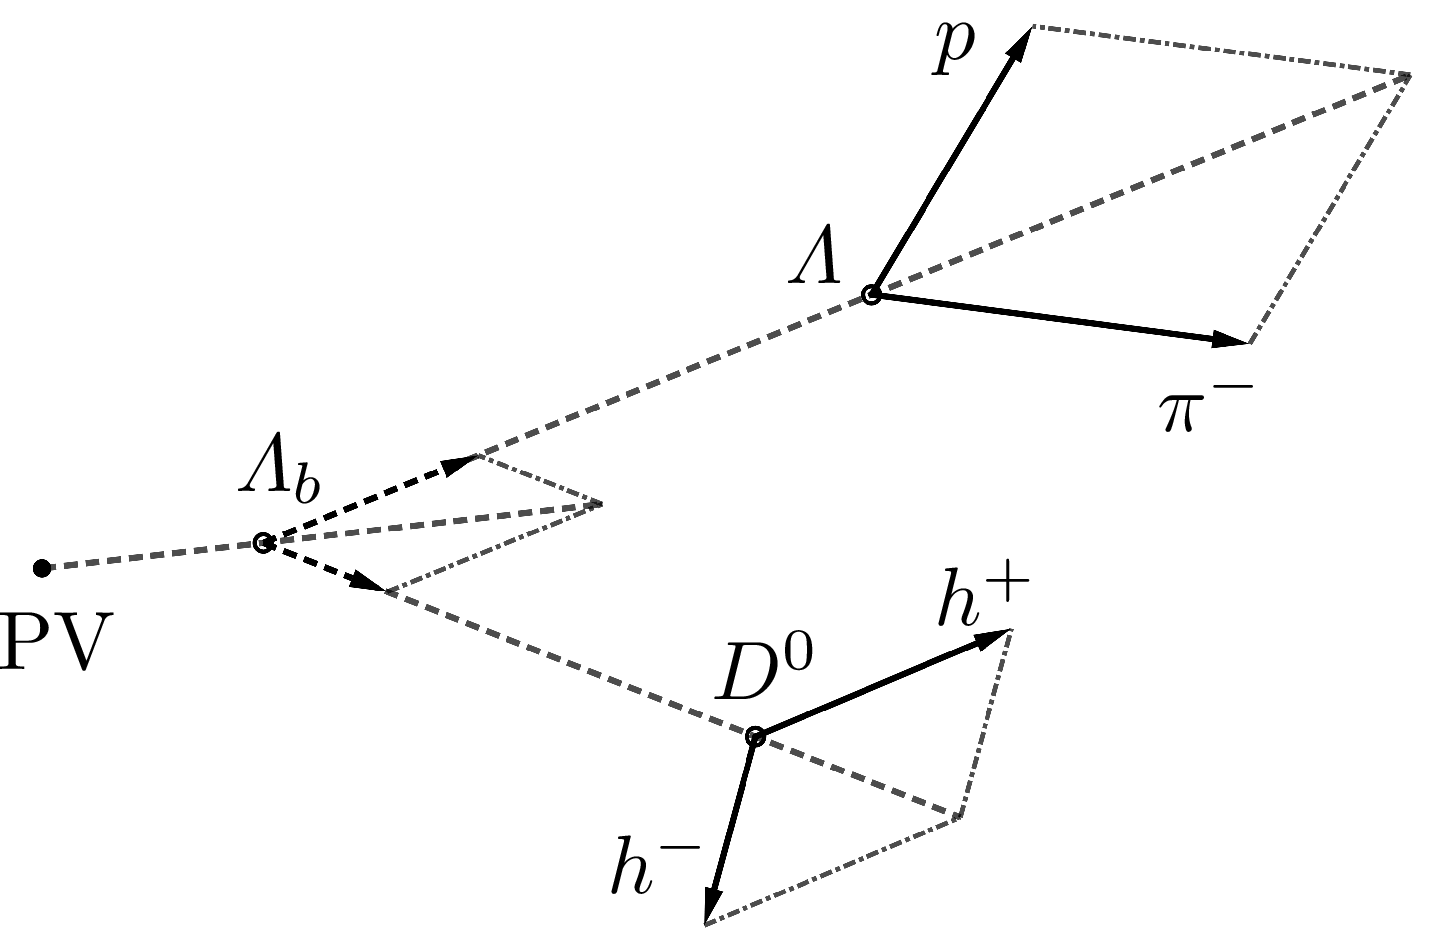
\includegraphics[scale=.12]{misc/dtf_Lb2DzLz.png}
        \caption{\decay{\Lb}{\Dz\Lz}}
    \end{subfigure}
    \begin{subfigure}{.49\textwidth}
        \centering
        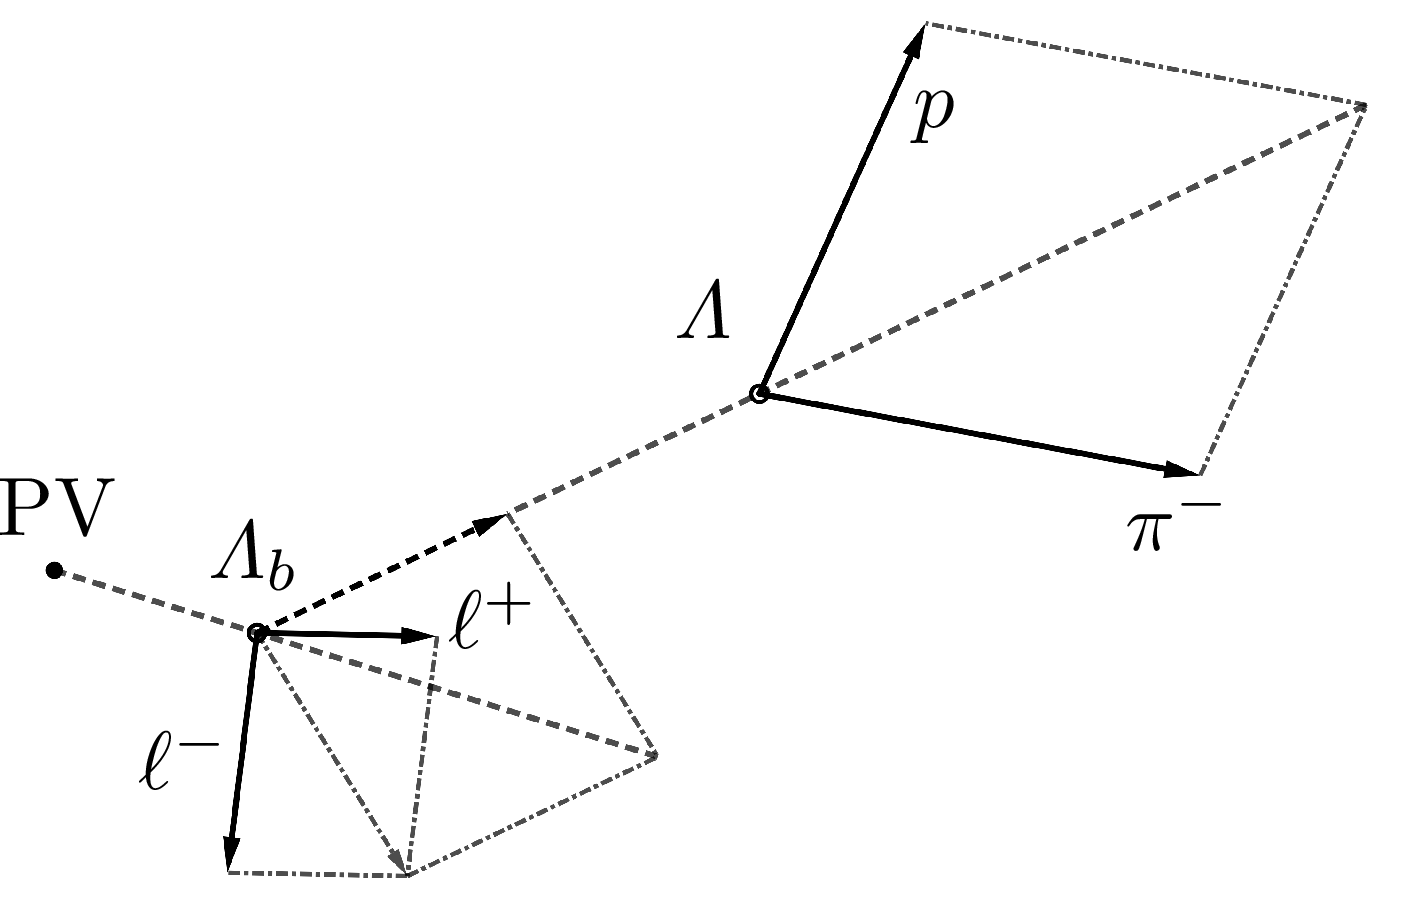
\includegraphics[scale=.12]{misc/dtf_Lb2JpsiLz.png}
        \caption{\decay{\Lb}{\jpsi\Lz}}
    \end{subfigure}
    \caption{Decay topologies as seen by a \gls{dtf} of the decays \decay{\Lb}{\Dz\Lz} (left) and \decay{\Lb}{\jpsi\Lz} (right). At \lhcb the \jpsi is a (short-living) resonance and the decay vertex of the \Lb baryon appears as a three-point vertex \decay{\Lb}{\ellp\ellm\Lz} during reconstruction (four \gls{dof} w/o \gls{pv} or mass constraints), whereas the flight lengths of the \Dz meson and \Lz baryon can be measured significantly and finite decay lengths can be accommodated in a \gls{dtf} (three \gls{dof} w/o \gls{pv} or mass constraints).}
    \label{fig:detector_decaytops}
\end{figure}

Constraining the mass of resonances, in general improves the resolution of related kinematic features, but does also introduce non-trivial distortions of background components.
For example, during the analysis of the background contribution of \decay{\Lb}{\Dz\proton\pim} decays in the invariant mass of \Dz and \Lz candidates, we discovered a dilution of the flight distance of \Lz candidates.
In case of genuine \decay{\Lb}{\Dz\proton\pim} decays, the distribution of the flight distance of \proton\pim combinations, spuriously forming a \Lz candidate, is symmetrically smeared around zero due to resolution effects in presence of no $m(\Lz)$ mass constraint and is uncorrelated with the invariant mass $m(\proton\pim)$ as shown in Fig.~\ref{fig:LbToDzppi_LzM_FDsig2}.
Constraining $m(\Lz)$ to its nominal value significantly increases the smearing and introduces a strong correlation between the flight distance and the invariant mass $m(\proton\pim)$ as shown in Fig.~\ref{fig:LbToDzppi_LzM_FDsig}. (Clearly, the latter has to be evaluated before applying the \gls{dtf} and forcing its value to the nominal value.)
The reason for this behavior is that a mass constraint (similar to a \gls{pv} constraint) affects the opening angle of the daughters of the \Lz candidate:
If the combined invariant mass of the \proton and \pim is below the constrained value of $m(\Lz)$, the \gls{dtf} pushes the three-momentum magnitudes towards larger values during the optimization.
A correlation with the decay tree of the corresponding \Dz is evaded by simultaneously increasing the opening angle between the three-momentum vectors which corresponds to an increase of the reconstructed flight distance.
Similarly, invariant masses above $m(\Lz)$ pushes the opening angle towards smaller values and thus decrease the reconstructed flight distance.
\begin{figure}[htbp]
    \centering
    \begin{subfigure}{.49\textwidth}
        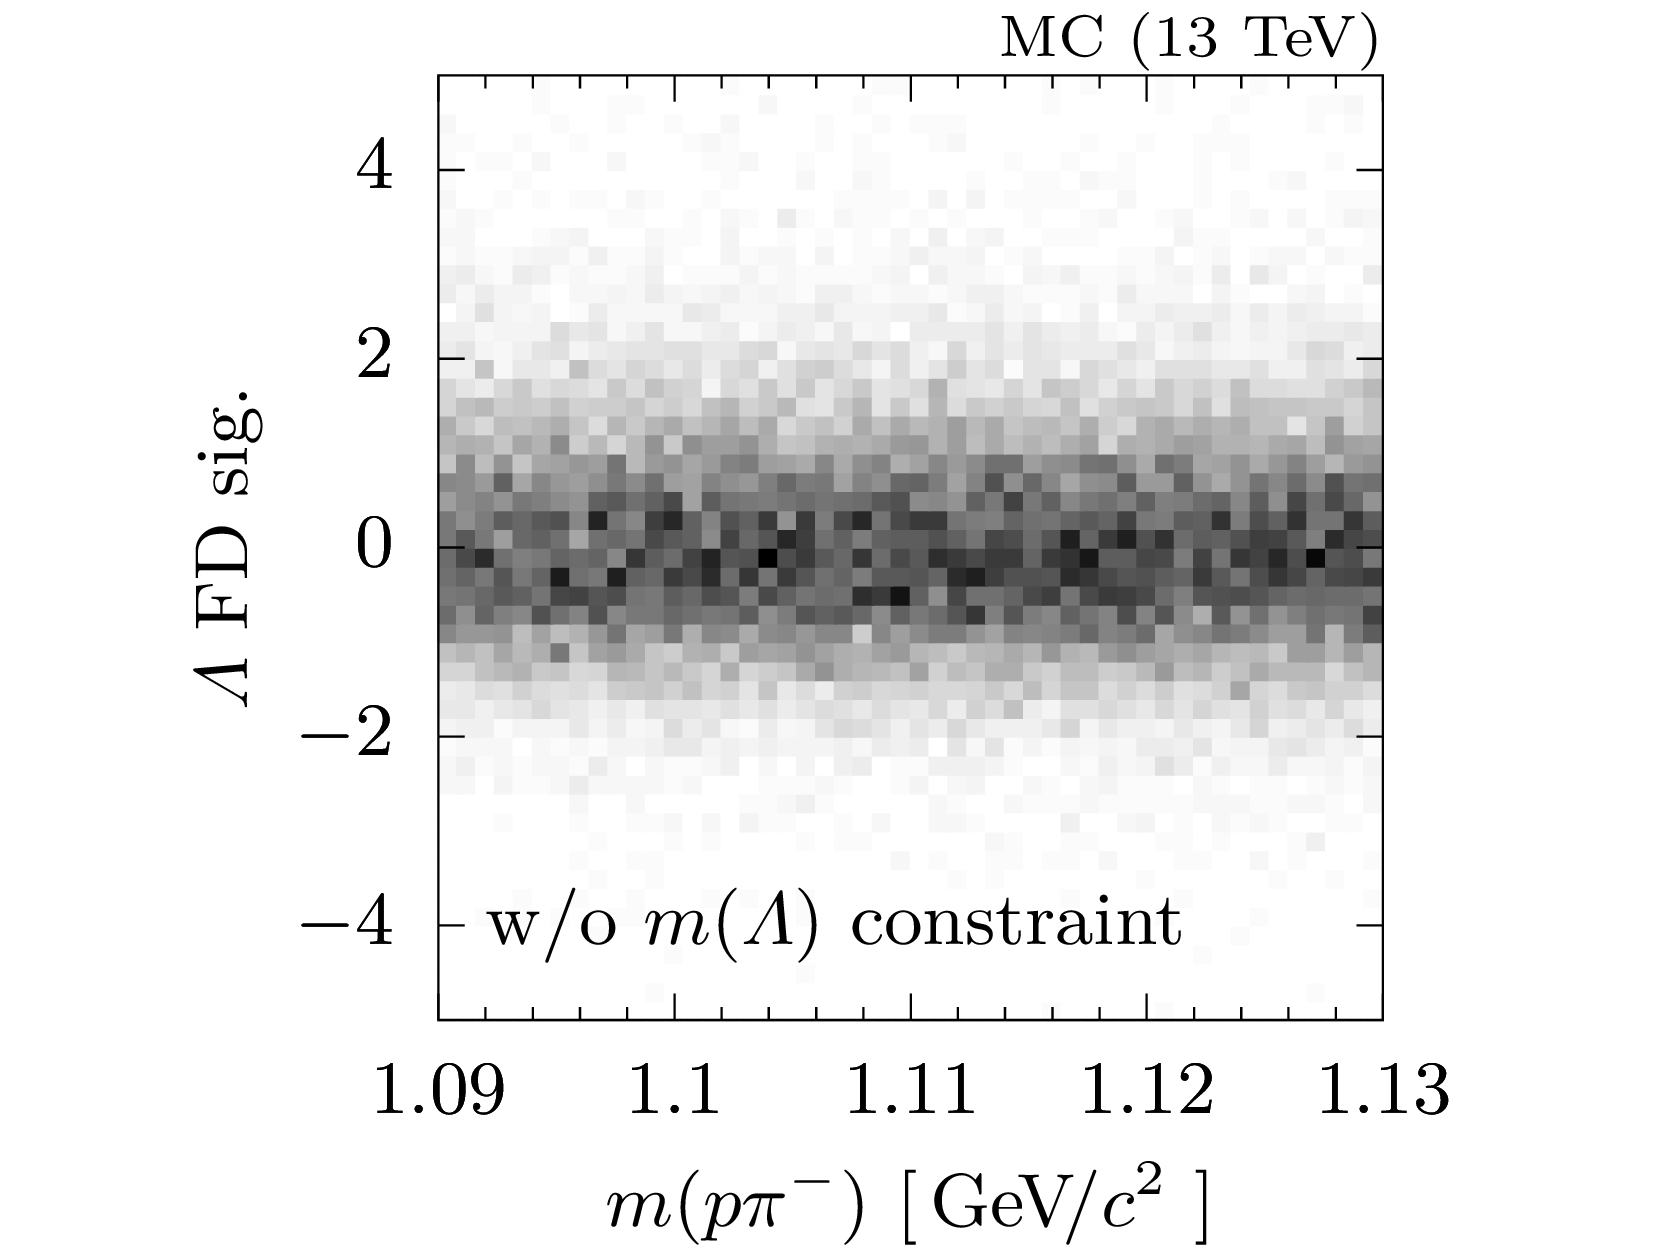
\includegraphics[scale=1.]{Lb2Dzppi_bkg/h2d_LzM_FDsig2.png}
        \caption{\Gls{dtf} without $m(\Lz)$ constraint.}
        \label{fig:LbToDzppi_LzM_FDsig2}
    \end{subfigure}
    \begin{subfigure}{.49\textwidth}
        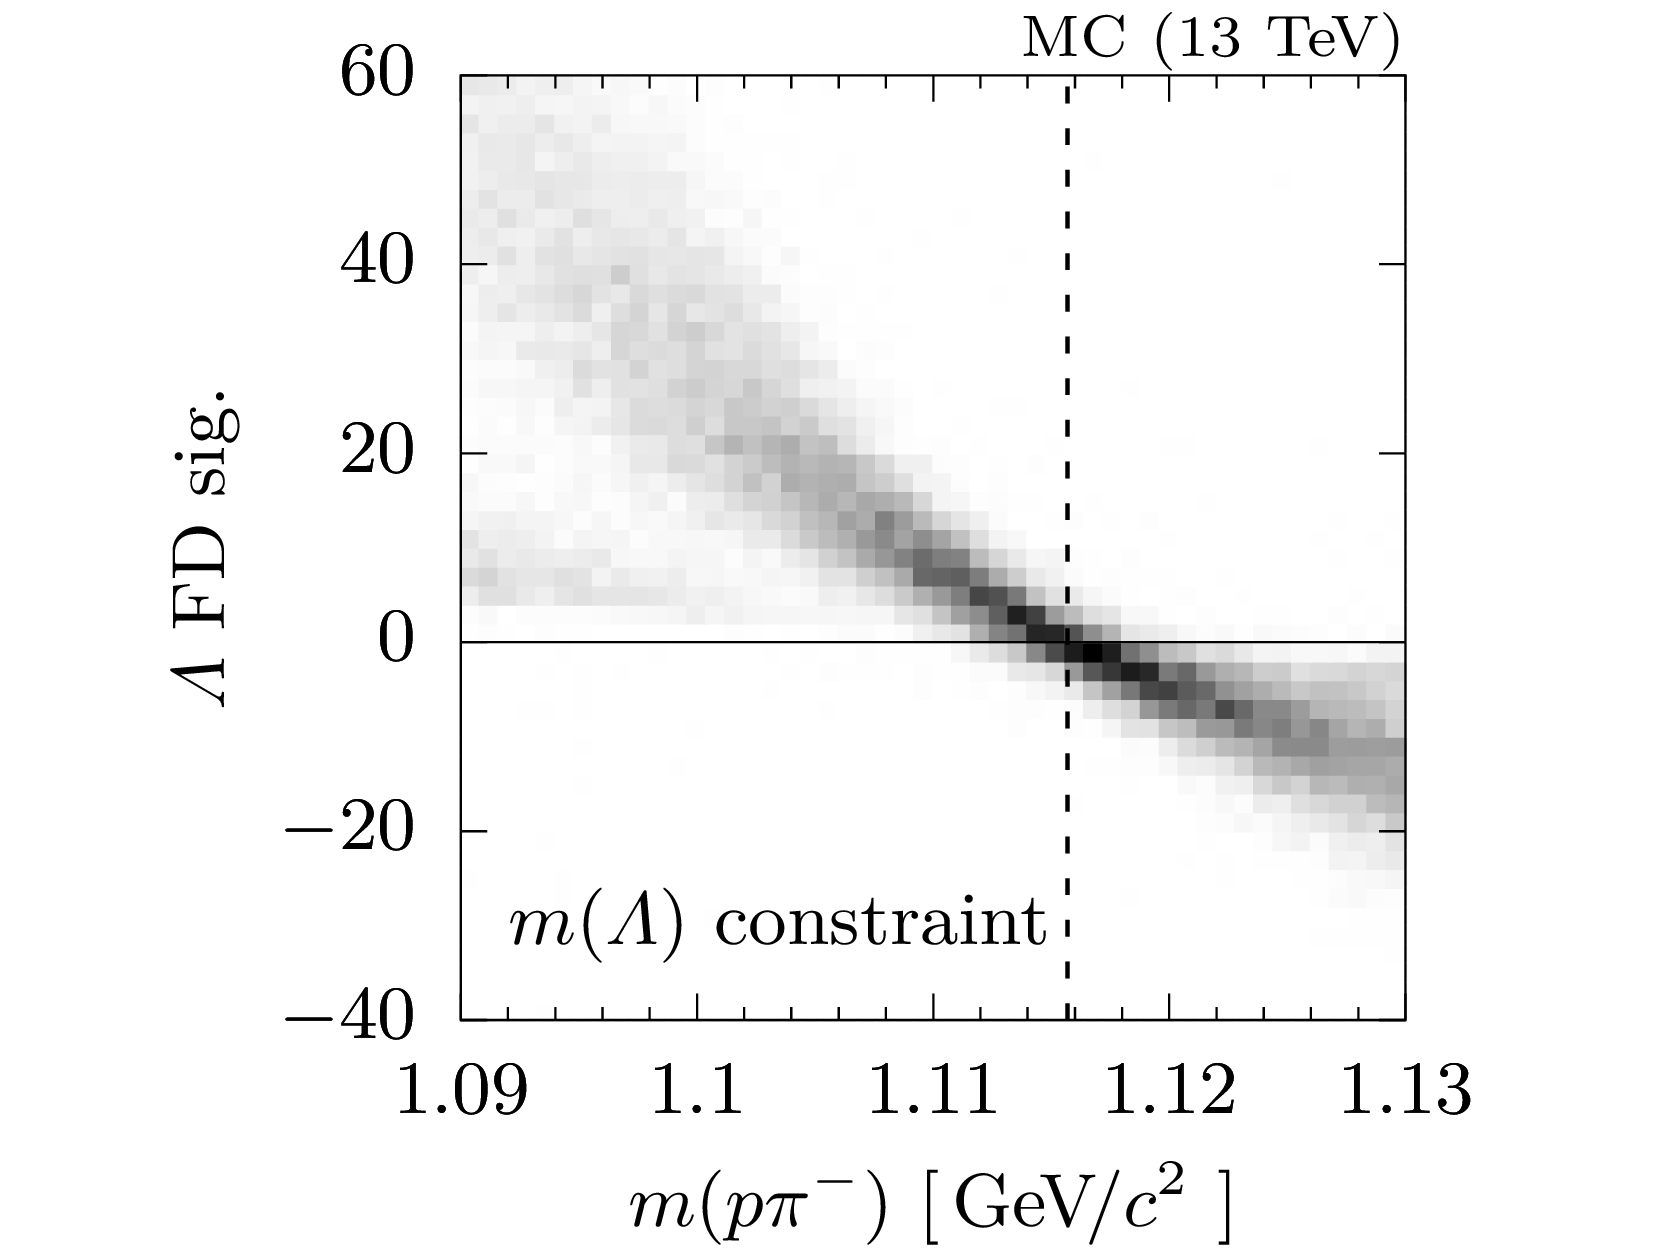
\includegraphics[scale=1.]{Lb2Dzppi_bkg/h2d_LzM_FDsig.png}
        \caption{\Gls{dtf} with $m(\Lz)$ constraint.}
        \label{fig:LbToDzppi_LzM_FDsig}
    \end{subfigure}
    \caption{Correlation of the combined invariant mass of \proton and \pim candidates of genuine \decay{\Lb}{\Dz\proton\pim} decays, reconstructed as \decay{\Lb}{\Dz\Lz} and the flight distance significance in presence of a \gls{dtf}. Constraining the invariant mass $m(\proton\pim)$ to $m(\Lz)$ (dashed line) introduces a significant correlation and increases the smearing of the flight distance distribution compared to the case of a \gls{dtf} without a $m(\Lz)$ constraint (left). (Note the different scaling of the $y$-axis.) The invariant mass shown on the $x$-axes (left and right) is the result of a four-momentum addition before applying the respective \glspl{dtf}.}
\end{figure}

In Fig.~\ref{fig:LbToDzppi_mLz_raw} we compare the effects of requiring a minimal flight distance and a minimal \gls{dtf} probability for the quoted example of the non-resonant background \decay{\Lb}{\Dz\proton\pim} in $m(\Dz\Lz)$.
The data are simulated \decay{\Lb}{\Dz\proton\pim} decays after a preselection step.
Before applying neither of both criteria, the distribution of the invariant mass is flat in good approximation.
Requiring a minimal \gls{dtf} probability symmetrically rejects events which are too far off the fixed $m(\Lz)$ value, whereas the flight distance criterion rejects only events above this value, resulting in the strongly asymmetric distribution we witnessed in Sec.~\ref{sec:bkgs_nonres}.
\begin{figure}[htbp]
    \centering
    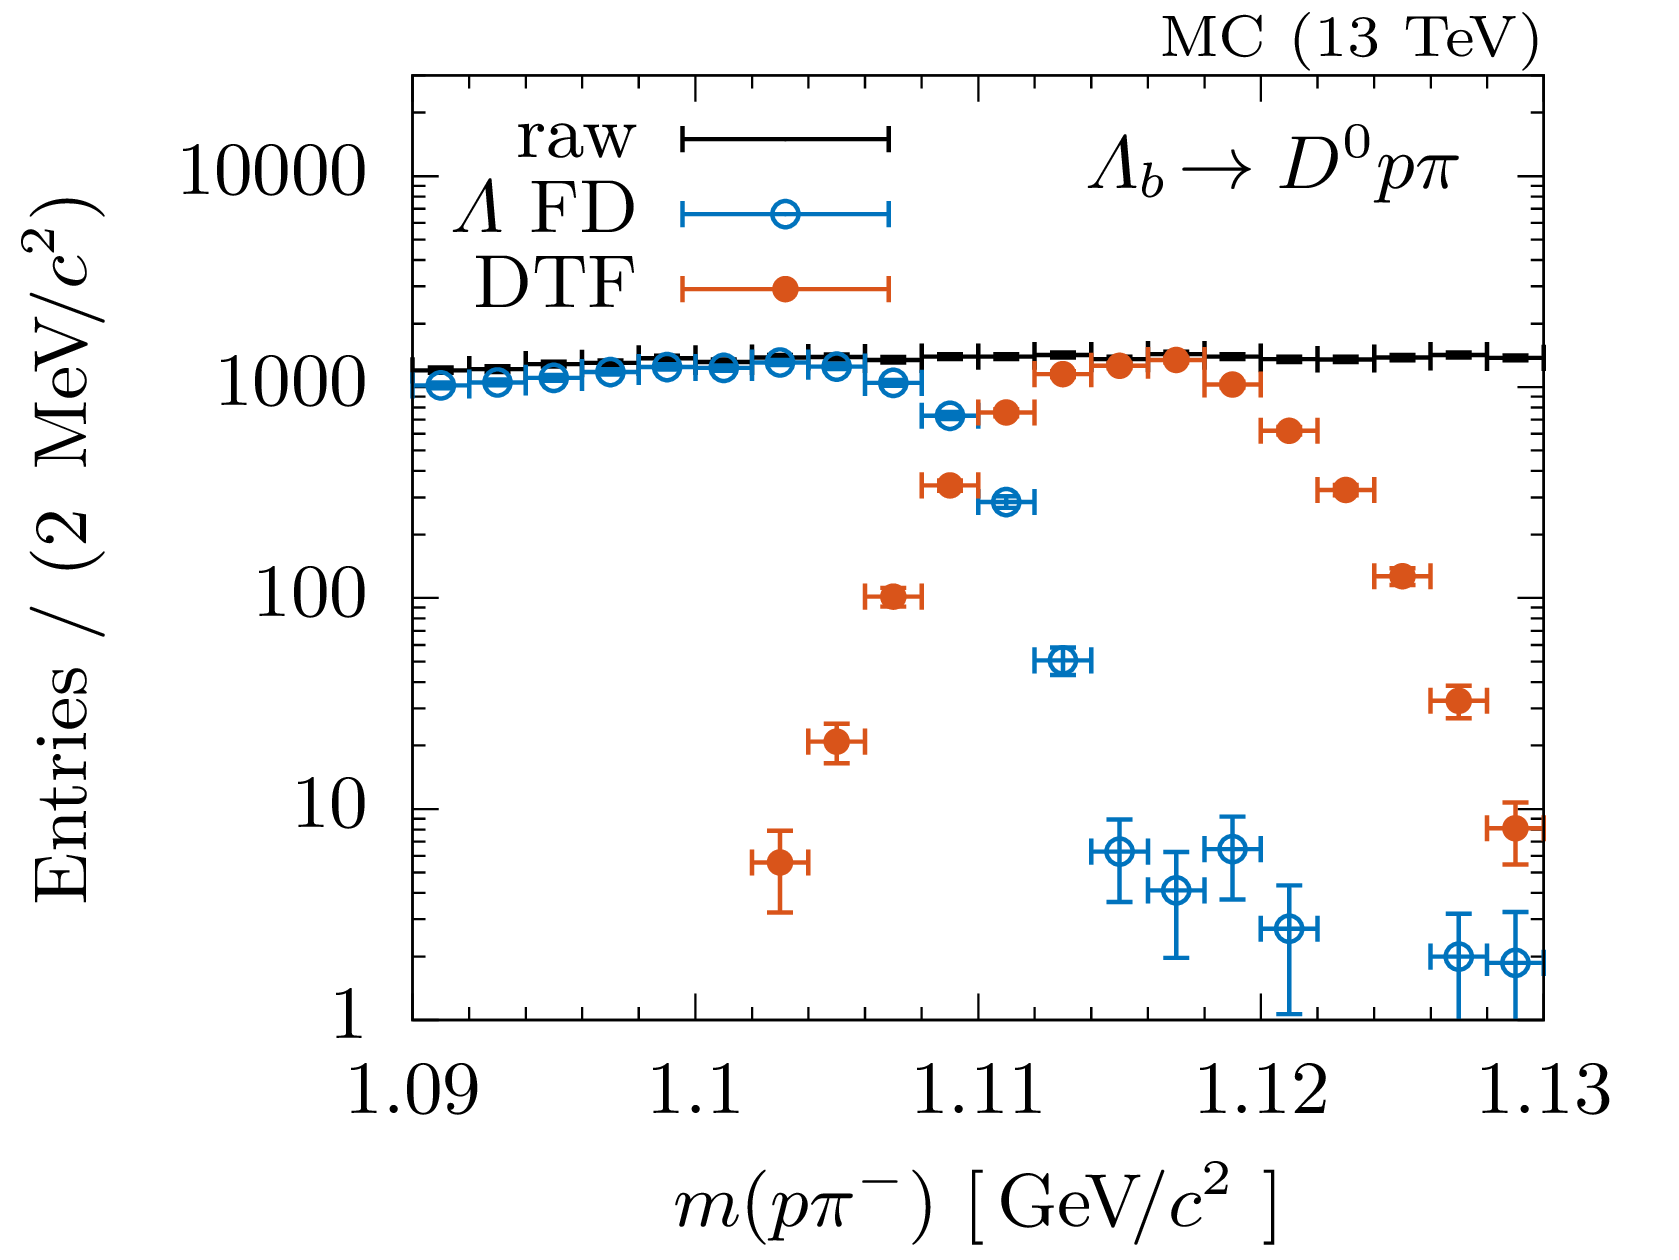
\includegraphics[scale=1.]{Lb2Dzppi_bkg/mLz_raw.png}
    \caption{Effect of requiring a minimal flight distance (\Lz FD) and a minimal \gls{dtf} probability (DTF) to simulated \decay{\Lb}{\Dz\proton\pim} decays that are reconstructed and fitted as \decay{\Lb}{\Dz\Lz} to the combined invariant mass of \proton and \pim candidates.}
    \label{fig:LbToDzppi_mLz_raw}
\end{figure}

